\section{Design}

\subsection{Database Design}
The project should have a database to store data. 
The data that should be stored in the database is something that 
resembles a batch. In the figure \ref{figure:eer_diagram_batch} it can be seen
what and how the data should be stored in the database.

The database is used in the system to keep track of data that resembles a batch's.
For example, if a person would like to know what happened then the beer was produced,
like what the highest temperature was it during the production, Did that have a
negative effect on the beer.
How many products were defect out of the total amount produced. 

\begin{figure}[ht]
\centering 
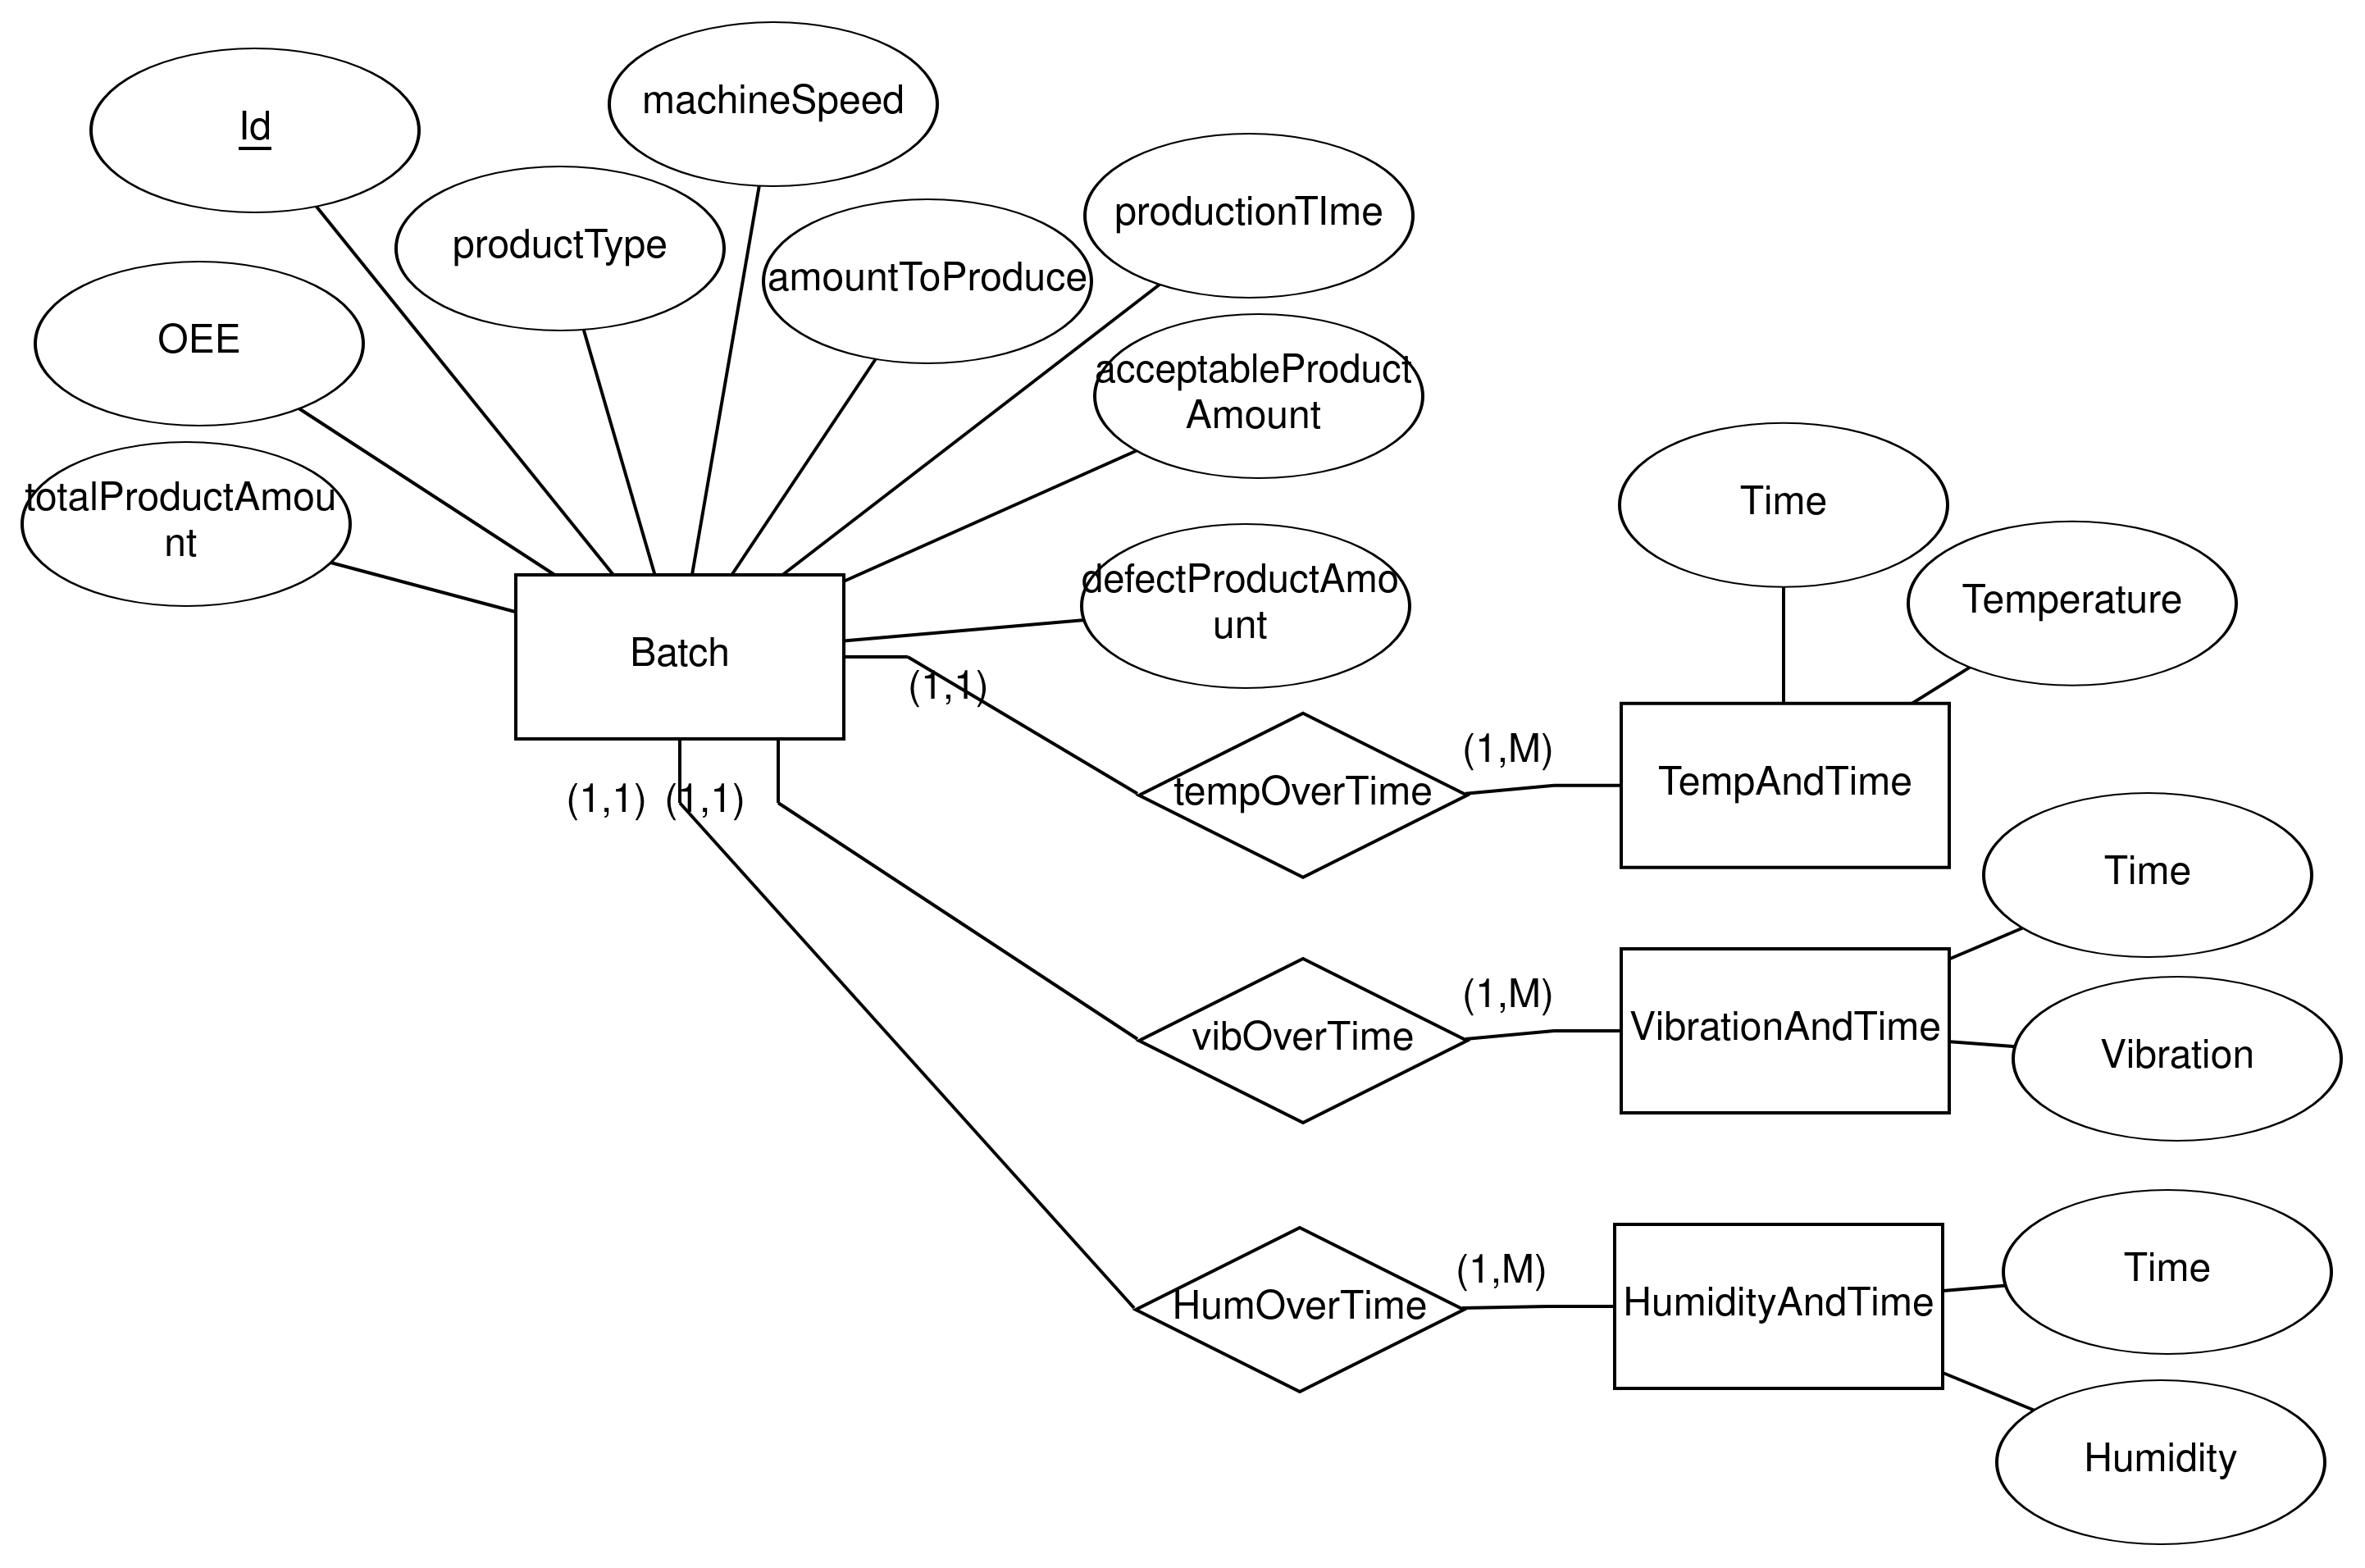
\includegraphics[width=0.8\linewidth]{images/eer_diagrams/database_EER_batch.png}
\caption{IR diagram for batch} 
\label{figure:eer_diagram_batch}
\end{figure}
